% Chapter Template

\chapter{Conclusion and outlook}\label{Chapter7} 

In this thesis searches for heavy neutral leptons in events with either three
charged leptons or displaced vertices are presented. The public
results can be found in References~\cite{Sirunyan:2018mtv} and~\cite{CMS-PAS-EXO-20-009} respectively.\\


The observation of neutrino flavor oscillations was one of the first 
definite experimental indications of the
presence of new physics not described by the SM theory. Thus, 
comprehand the mechanism that discloses the neutrino mass would be a
vital flare into BSM physics. Therefore, it felt crucial to investigate at the LHC
experiments the signatures of different neutrino mass models
to try spotting the mysterious new physics.\\
The two results presented in the dissertation cooperate in the arduous attempt of confronting exotic BSM
models with the experimental data. The aspiration is to find new
physics able to describe the unexplained
physics observations not covered by the SM. 

We decided to focus on right-handed (RH) neutrino or heavy neutral lepton (HNL)
model. The introduction of massive RH
neutrinos provides an answer to the SM problem of the
neutrino masses via a type-I seesaw mechanism.  
In Chapters~\ref{Chapter1} and~\ref{Chapter3} we illustrated
the relevance and the interest for the
ongoing HNL search program, describing first the theory setting 
and then mentioning the various of experiments and results
focusing on HNL.\\
When we hypothesize a new particle as RH neutrinos, $N_{I}$, we
are interested in their properties like the mass $M_I$ of the HNLs and
their mixing parameter, $|V_{\alpha I}|^2$  with the SM neutrino of flavor $\alpha$,
controlled by the Yukawa coupling $F_{\alpha I}$. The values of $|V_{I
  \alpha}|^2$ is unknown and the experimental
sensitivity for both the two analyses presented here is expressed in
terms of the coupling $|V_{\alpha I}|^2$
as a function of $M_I$ for a given flavor $\alpha$. 

Furthermore we introduced a list of direct HNL search results; we give an overview
of the experimental current and past landscape describing the different decay modes and
mass ranges that are targeted by the single measurement.
The strategies in direct HNL searches depend greatly on the mass
which we desire investigating. For $M_{I} > 5$\GeV, \hnl can be
produced uniquely at either LHC or at similar energy colliders, via a few
mechanisms (vector boson fusion, s-channel exchange of virtual
W-bosons or in real gauge boson decays) according to the production
energy and \hnl mass. For $M_{I} < 5$\GeV, we recur to b-factories
or fixed target experiments. \\
Special attention is paid to lepton and hadron collider
searches. The LEP results from DELPHI happen to be the best results at
low mass from collider experiment up to the publication of the results
of this dissertation. The outstanding sensitivity al low mass from
$e^{+}e^{-}$ data was surely a good motivation to invest a quite
important effort to extend as well the low mass sensitivity of
the CMS experiment.\\

Chronologically we have focused first on the
moderate and high mass search to migrate to very low mass search which
necessarily requires the inclusion of displaced scenarios.

During my first PhD year, I worked on the ``search for heavy neutral leptons in events with three charged
 leptons in proton-proton collisions at $\sqrt{s}$ =
 13\TeV''~\cite{Sirunyan:2018mtv}. It was not observed any
 statistically significant excess of signal events over the expected
SM background. At 95\% confidence level upper limits were set on the mixing
parameters \mixpare and \mixparm. The excluded values are in the
ranges between $1.2\times 10^{-5}$ and $1.8$ for masses included
between 1\GeV $< m_\hnl <$ 1.2\TeV. 
These were the first direct limits for HNL masses above 500\GeV and the first
limits obtained at hadron colliders for HNL masses below 40\GeV.
At large HNL masses, the results improved those previously published
by the ATLAS~\cite{Aad_2015} and CMS~\cite{Khachatryan_2015,Sirunyan:2018xiv}
experiments. 

The remaining time of my PhD was dedicated to the ``Search for long-lived heavy neutral leptons with displaced
vertices in pp collisions at $\sqrt{s}$ =
 13\TeV''~\cite{CMS-PAS-EXO-20-009}. The data were collected from the
CMS experiment in years 2016 -- 18 corresponding to an integrated
luminosity of 137\fbinv.
The signature consists of one prompt charged lepton and two displaced
charged leptons in any flavor combination of electrons
and muons. Two interpretations are proposed considering on one hand uniquely the
Dirac HNL nature, on the other hand the Majorana HNL nature. 
No statistically significant deviation from the expected
SM background was observed. At 95\% confidence level limits were set on the mixing
parameters \mixpare and \mixparm.
The excluded values are in the
ranges between $3\times 10^{-7}$ and $1\times 10^{-3}$ for masses included
between 1\GeV $< m_\hnl <$ 15\GeV. \\

The opportunity to work on such complementary analyses
allowed me to gain over the years considerable expertise in HNL
searches with multilepton final states at CMS.\\
Remarkable were the LL-HNL workshops to which I have actively
partecipated. They gave the chance to explore the 
state-of-the-art of HNL models and results in particular with LLP
signatures~\cite{Alimena_2020}. Furthermore we identified new open questions and
we emphasize the priority 
of complementary and synergetic searches; these discussions
led to the formulation of new searches and new opportunities
for discovery.\\

In the next section the latest sensitivity
estimations and incoming experimental results are presented. Finally
it is given 
an overview of possible future experiments
and detector upgrades. 


\section{Outlook}
Abundantly clear at this point of the thesis, HNLs are one of the most
exciting and best-motivated potential solutions for some of the
outstanding problems of the SM. However, if they happen to exist, their
Majorana/Dirac natures, their masses, and their coupling with the SM
neutrinos are far from obvious and clear. Thus we need to adopt a
comprehensive and vast approach in seeking for HNL probing heavy
neutral leptons with MeV- and TeV-scale masses.\\

For HNLs in the GeV-TeV mass ranges, we enter the domain of the
particle colliders and we are looking for prompt HNLs produced via charged current (CC) Drell-Yan
process, via gluon fusion, and via $\PW \gamma$ fusion. 
In this part of phase space we find a few new results a several
promising new searches.

Recently at CMS it has been carried out a search for right-handed bosons ($\PW_R$
and RH neutrinos in the left-right symmetric model extension of the
SM~\cite{CMS-PAS-EXO-20-002} using pp collisions data collected at $\sqrt{s}$ =
 13\TeV and corresponding to 137\fbinv integrated luminosity. The
 signature consists of events with two same-flavor light leptons and
 two quarks. For $m_\hnl = m_{\PW_{R}}/2$ ($m_\hnl = 200$\GeV) the
 mass of the $\PW_R$ is excluded at 95\% CL up to 4.7 (4.8) and 5.0 (5.4) TeV for the electron and muon
channel, respectively. 

At the time of the publication of the analysis presented in
Chapter~\ref{Chapter5}, the results were positively received by the community and highly appreciated
for the big effort was put into widening the mass range and
improving the sensitivity previously obtained. The
data were corresponding to an integrated luminosity of only to
35.9\fbinv collected in 2016. Thus it is necessary to perform the same
search on the full available dataset which corresponds to an integrated luminosity of 
137\fbinv. \\
The analysis is being carried out by a Ugent colleague (L. Wezenbeek)
who not only is integrating with the fullRun2 but he is also improving
some selection strategy aspects to increase the quality of the final
results. In particular, if we recal well, one of the largest
background of~\cite{Sirunyan:2018mtv} is the one coming from nonprompt
leptons. The updated lepton ID makes use of a new machine learning
based lepton identification algorithm which was developed to be
optimal at rejecting nonprompt leptons~\footnote{This machine learning
based lepton identification algorithm was devoped in the context of
the $t\overline{t}H$ analysis~\cite{Sirunyan_2018_ttH} and further improved at UGent by Willem
Verbeke and deploied later in the following outstanding
analsyses~\cite{CMS:2018sgc_tzq, Sirunyan_2021_higgsmumu}.}. The algorithm exploits the
characteristcs of the jet containing the lepton, and puts together all
variables that discriminate between prompt and
nonprompt leptons with a machine learning algorithms. The results is
that using the new ID instead of the priors, there is an increase in effciency
per lepton of 20\% and for the same signal
effciency there is a reduction of the
nonprompt background
by factor 10\%. Although the rest of the analysis workflow is going to be very
similar to what published in 2018, the advancements done in reducing the
major background, possible progresses in signal categorization and the
triple amount of data will bring sizable change in the final
sensitivity.

In the same analysis framewrok and timeline, a new exciting addition
is going to be included. For the first time at CMS, the mixing between
HNL and tau neutrinos is going to be probed. In
Figure~\ref{fig:HNL_bc8_pbc_2} is indisputable the need to dedicate
some effort in searches sensitive to tau coupling, \mixpart. The
ongoing analysis will look for HNL in events with either one light leptons
and two taus or two light leptons and one $\tau$. The consider mass
range is between 20\GeV and 1\TeV. The main difficulties of these final
states are on one hand trying to reduce the considerable nonprompt tau background and
improve the S/B ratio; on the other hand dealing with quite large tau
\pt thresholds which automatically exlcude a part of the phase space
reducing the selection acceptance. \\
Despite the numerous challenges, esitmating the limits for \mixpart is
one of the most important piece of the big HNL puzzle and long waited
by the theory comunity.  

For future very high HNL mass searches, an interesting suggestion comes from
the work presented in Ref.~\cite{Pascoli_2019}. It is considered the
final state $\hnl \ell + X\rightarrow 3\ell + \ptmiss + X$. The
authors use as major
discriminant tecniques a dynamic
jet veto (\ie it depends on the \pt of the hightest \pt lepton) and a
requirement on the scalar sum of three leptons \pt. At 14\TeV, it appears that
the proposed analysis strategy can
improve sensitivity by an order of
magnitude for $m_\hnl > 150$\GeV at $\mathcal{L} = 300$\fbinv and
3\abinv. \\

Figures~\ref{fig:HNL_bc6_pbc_2} and~\ref{fig:HNL_bc7_pbc_2} show that
the HNL mass range between 1\GeV and 20\GeV is one the most contend phase
space by so many different present and future experiments. This
results in a quite vigorous competition as well as in a very driving
experimental enviroment. The analysis presented in Chapter~\ref{Chapter6} sits excalty there. \\
Thus it is evident the necessity of exploring almost one by one the
other players with great attention paid to future results and experiments.

In the long-lived HNL scenario, the channel with hadronic \PW decay
can also be probed. The analysis is being carried out by a Ugent
colleague (B. Vermasse). A search for HNL is performed using the pp collision
data at a $\sqrt{s}$ = 13\TeV, collected by the CMS detector during Run
2. The search targets final states with a prompt lepton, a displaced lepton, a
displaced jet and a secondary displaced vertex. The machine
learning technique, called Particle Flow Network is deployed to
improved the separation between signal and background.
Separate PFN trainings
are performed, four for 1\GeV $< m_\hnl < 4$\GeV hypothesis and four for $m_\hnl > 4$\GeV hypothesis.
The output of the PFN classifier is used together with the
displacement of the SV and its mass to categorized the search regions.
The estimation of the SM background appears to be challenging for
similar reasons as the ones explored in this dissertation. The
analyzers are going to estimate the background contribution using a data-driven 
technique and then validate it make use of data control region. The
final sensitivity will be presented in the 2D \mixpar -- $m_\hnl$
plane as for the three lepton final state analyses.

\begin{wrapfigure}{l}{0.5\textwidth}
\centering
    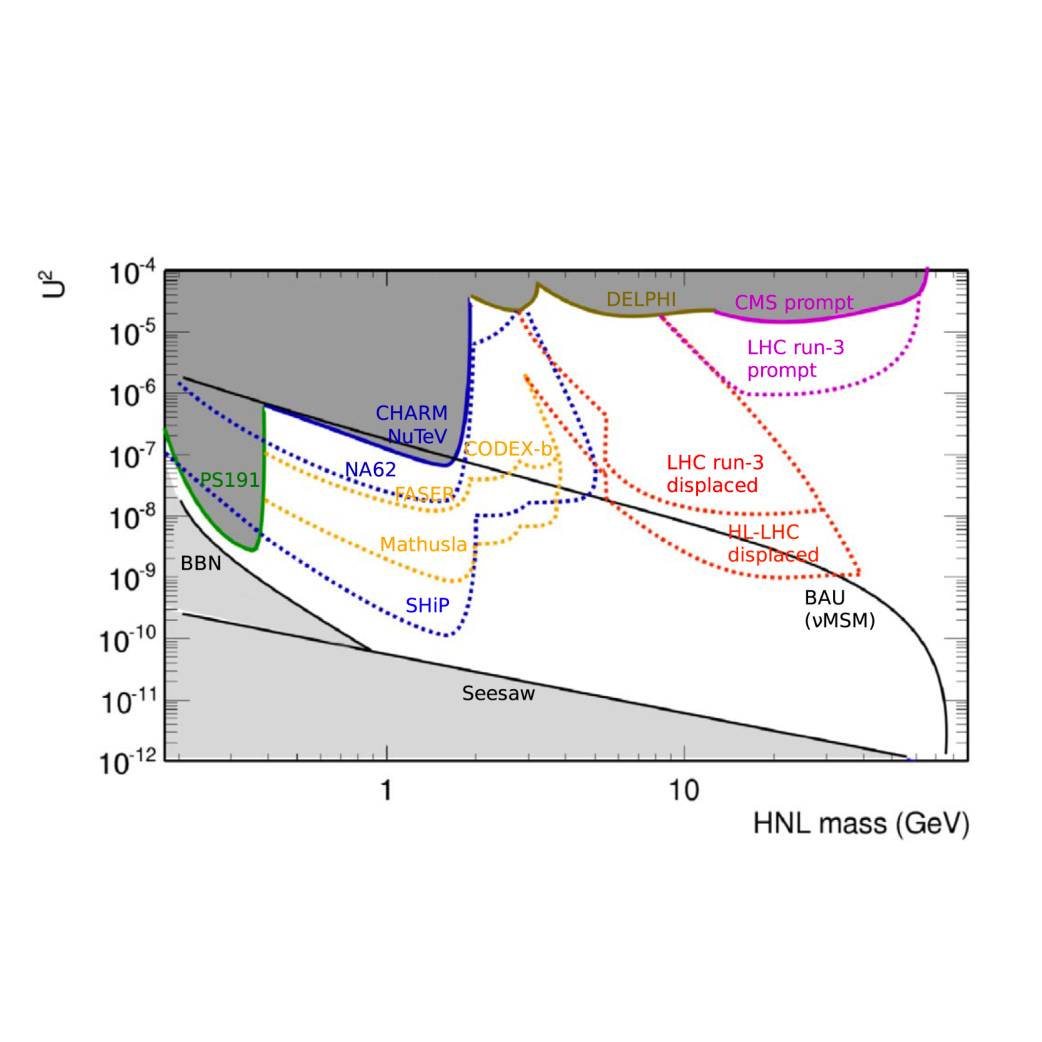
\includegraphics[clip,trim=0.5cm 3.5cm 1.cm 3cm, width=.48\textwidth]{Figures/c7/projection_alimena.pdf}
\caption{ ~\cite{Alimena_2020}}
\label{fig:atlas}
\end{wrapfigure}



\paragraph{Displaced HNL -->}
\begin{itemize}
\item Marco's projection for 3\abinv --> HL-LHC
\end{itemize}
Figure 7 in ~\cite{Alimena_2020}

\paragraph{Detector upgrade -->}
\begin{itemize}
\item CMS timing detectors: tracker,  CMS MTD Endcap Timing Layer,
  ~\cite{CERN-LHCC-2017-027} and muon system 
\item trigger upgrade
\end{itemize}

\paragraph{new experiments -->}
\begin{itemize}
\item mathusla200,
\item ship
\item NA62
\item codex
\end{itemize}






\vspace {5cm}








%%%%%%%%%%%%%%%%%%%%%%





